\documentclass[12pt]{article}

\usepackage{graphicx}
\usepackage{amsmath}
\usepackage{amssymb}
\usepackage{natbib}
\usepackage{amsfonts}
\usepackage{multicol}
\usepackage{float}
\usepackage{oldgerm}
\usepackage{bm}
\usepackage{mathtools}
\usepackage{wrapfig}
\usepackage{fancyhdr}
\usepackage[export]{adjustbox}
\usepackage{xcolor}
\usepackage[shortlabels]{enumitem}

\pagestyle{empty}

\setlength{\headsep}{0.5cm}
\setlength{\oddsidemargin}{-0.5cm}
\setlength{\textwidth}{16.5cm}
\setlength{\textheight}{24cm}
\voffset = -2cm


\pagestyle{fancy}
\fancyhf{}
\rfoot{
\includegraphics[width=1.0in]{cnm.png}}
\lfoot{ENGR2910 - Midterm 1}
\setlength\parindent{0pt}
\begin{document}

\begin{center}
\hfil
{\large\bf {ENGR 2910-101: Circuit Analysis}}
\hfill Instructor: Brian Rashap\\
Midterm 1  \hfill Due: 02/15/23\\
\hrulefill\\
\end{center}

Please show all your work and circle your answers to each question.
\newline\newline

{\bf Question 1} [10]
\newline
What is the value of $v_2$?

\begin{figure}[h!]
\centering 
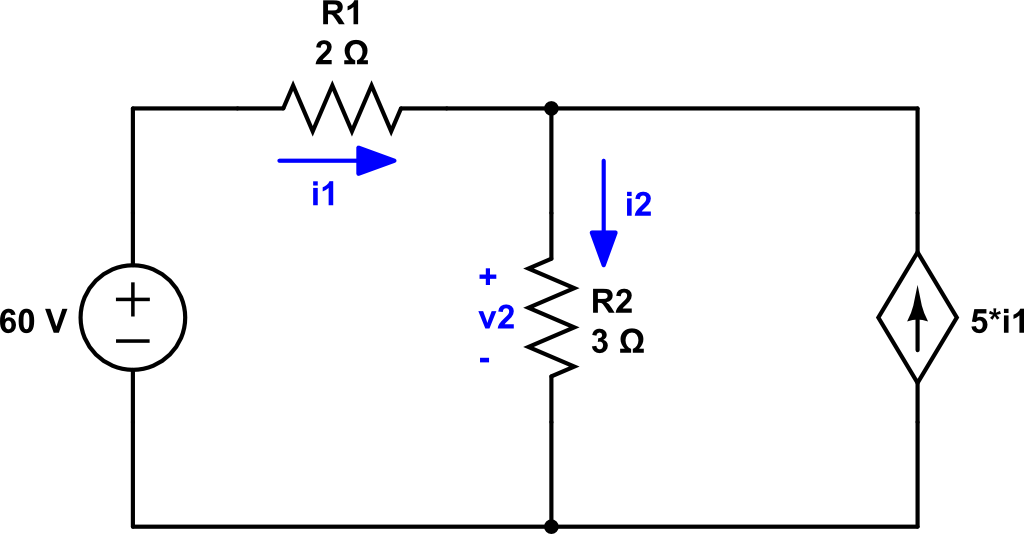
\includegraphics[clip,width=0.49\textwidth]{mid1_1.png}
\end{figure}

{\bf Question 2} [10] 
\newline
What is the equivalent resistance between $A$ and $B$?

\begin{figure}[h!]
  \centering 
 \vspace{-0.1in}
 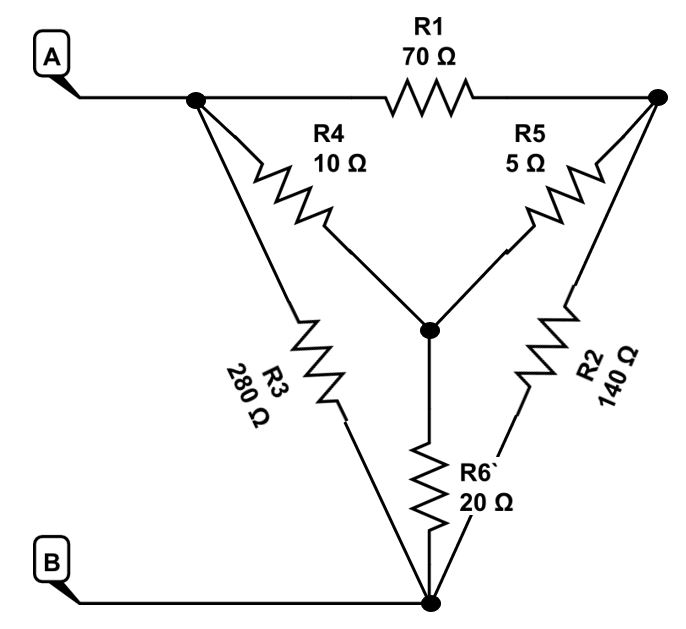
\includegraphics[clip,width=0.49\textwidth]{mid1_2.jpg}
\vspace{-0.1in}
\end{figure}


\newpage
{\bf Question 3} [20] 
\newline
For the below circuit:

\begin{figure}[h!]
     \centering
\vspace{-0.1in}
       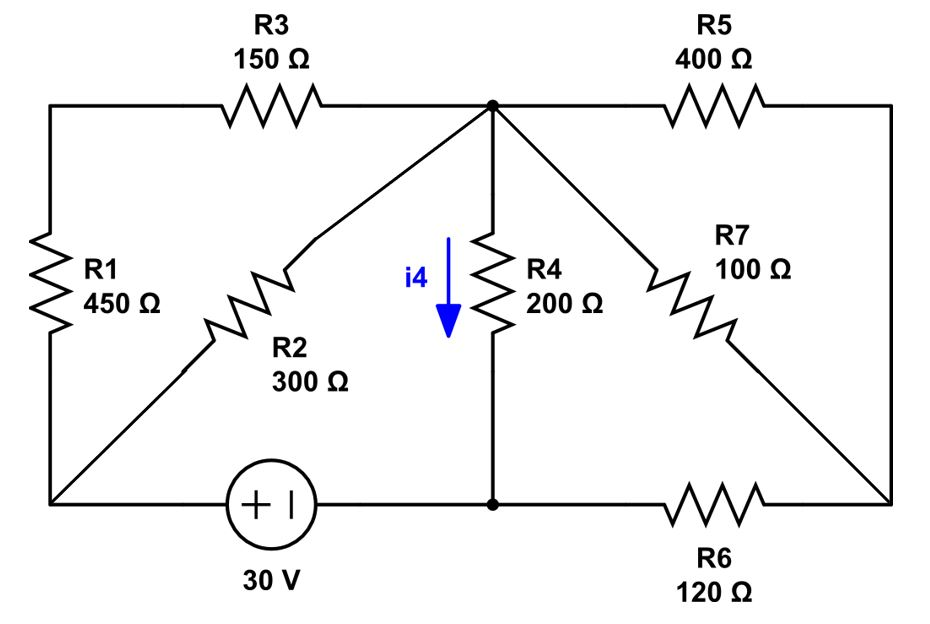
\includegraphics[clip,width=0.6\textwidth]{mid1_4.jpg}
\vspace{-0.15in}
\end{figure}

\begin{enumerate}[(a)]
\item What is the equivalent resistance seen by the voltage source (30V)?
\item What is the current $i_4$?

\end{enumerate}


{\bf Question 4} [20] 
\newline
Consider the voltage divider below (both with and without a load):

\begin{figure}[!h]
  \centering 
  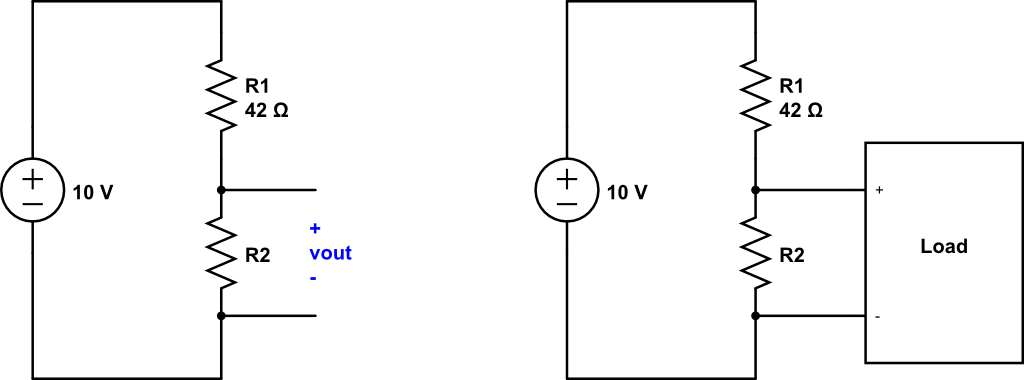
\includegraphics[clip,width=0.6\textwidth]{mid1_3.png}
\end{figure}

\begin{enumerate}[(a)]
\item Without a load, what value of $R_2$ will provide a $v_{out}$ of $3V$?
\item If the load has has a resistance of $9 \Omega$:
\begin{enumerate}[(i)]
\item For the $R_2$ above, how does $R_1$ need to change to maintain proving $3V$ to the load?
\item How much Power is being absorbed by the load?
\item How much Power is being provided by the $10V$ source?
\end{enumerate}
\end{enumerate}
\newpage

{\bf Question 5} [40]
\newline
For the following circuit:

\begin{figure}[h!]
\centering 
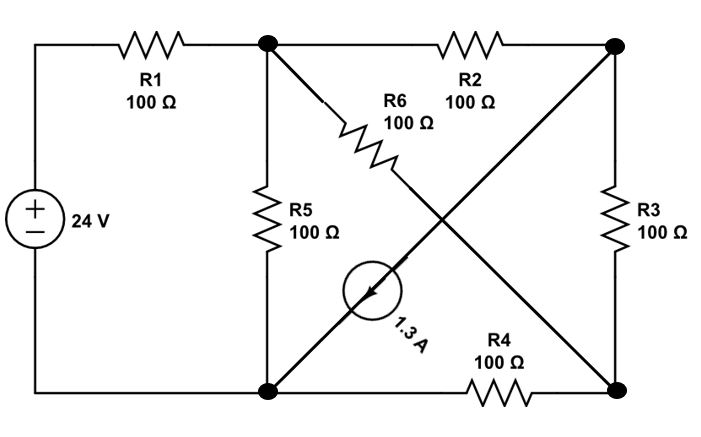
\includegraphics[clip,width=0.6\textwidth]{mid1_5.jpg}
\end{figure}



\begin{enumerate}[(a)]
\item How many essential nodes ($n_e$)?
\item How many essential branches ($b_e$)?
\item List the essential branches.
\item Using the Node-Current Method, how many KCL equations are needed?
\item How many KVL equations are needed?
\item Write out the Node-Current Matrix (DO NOT SOLVE IT).

\end{enumerate}

{\bf Extra Credit}

What was the Max Salazar building named after?


\end{document}
